\documentclass{standalone}
\usepackage{tikz}
\usetikzlibrary{patterns, positioning}
\usepackage[sfdefault]{ClearSans} %% option 'sfdefault' activates Clear Sans as the default text font
\usepackage[T1]{fontenc}

\begin{document}
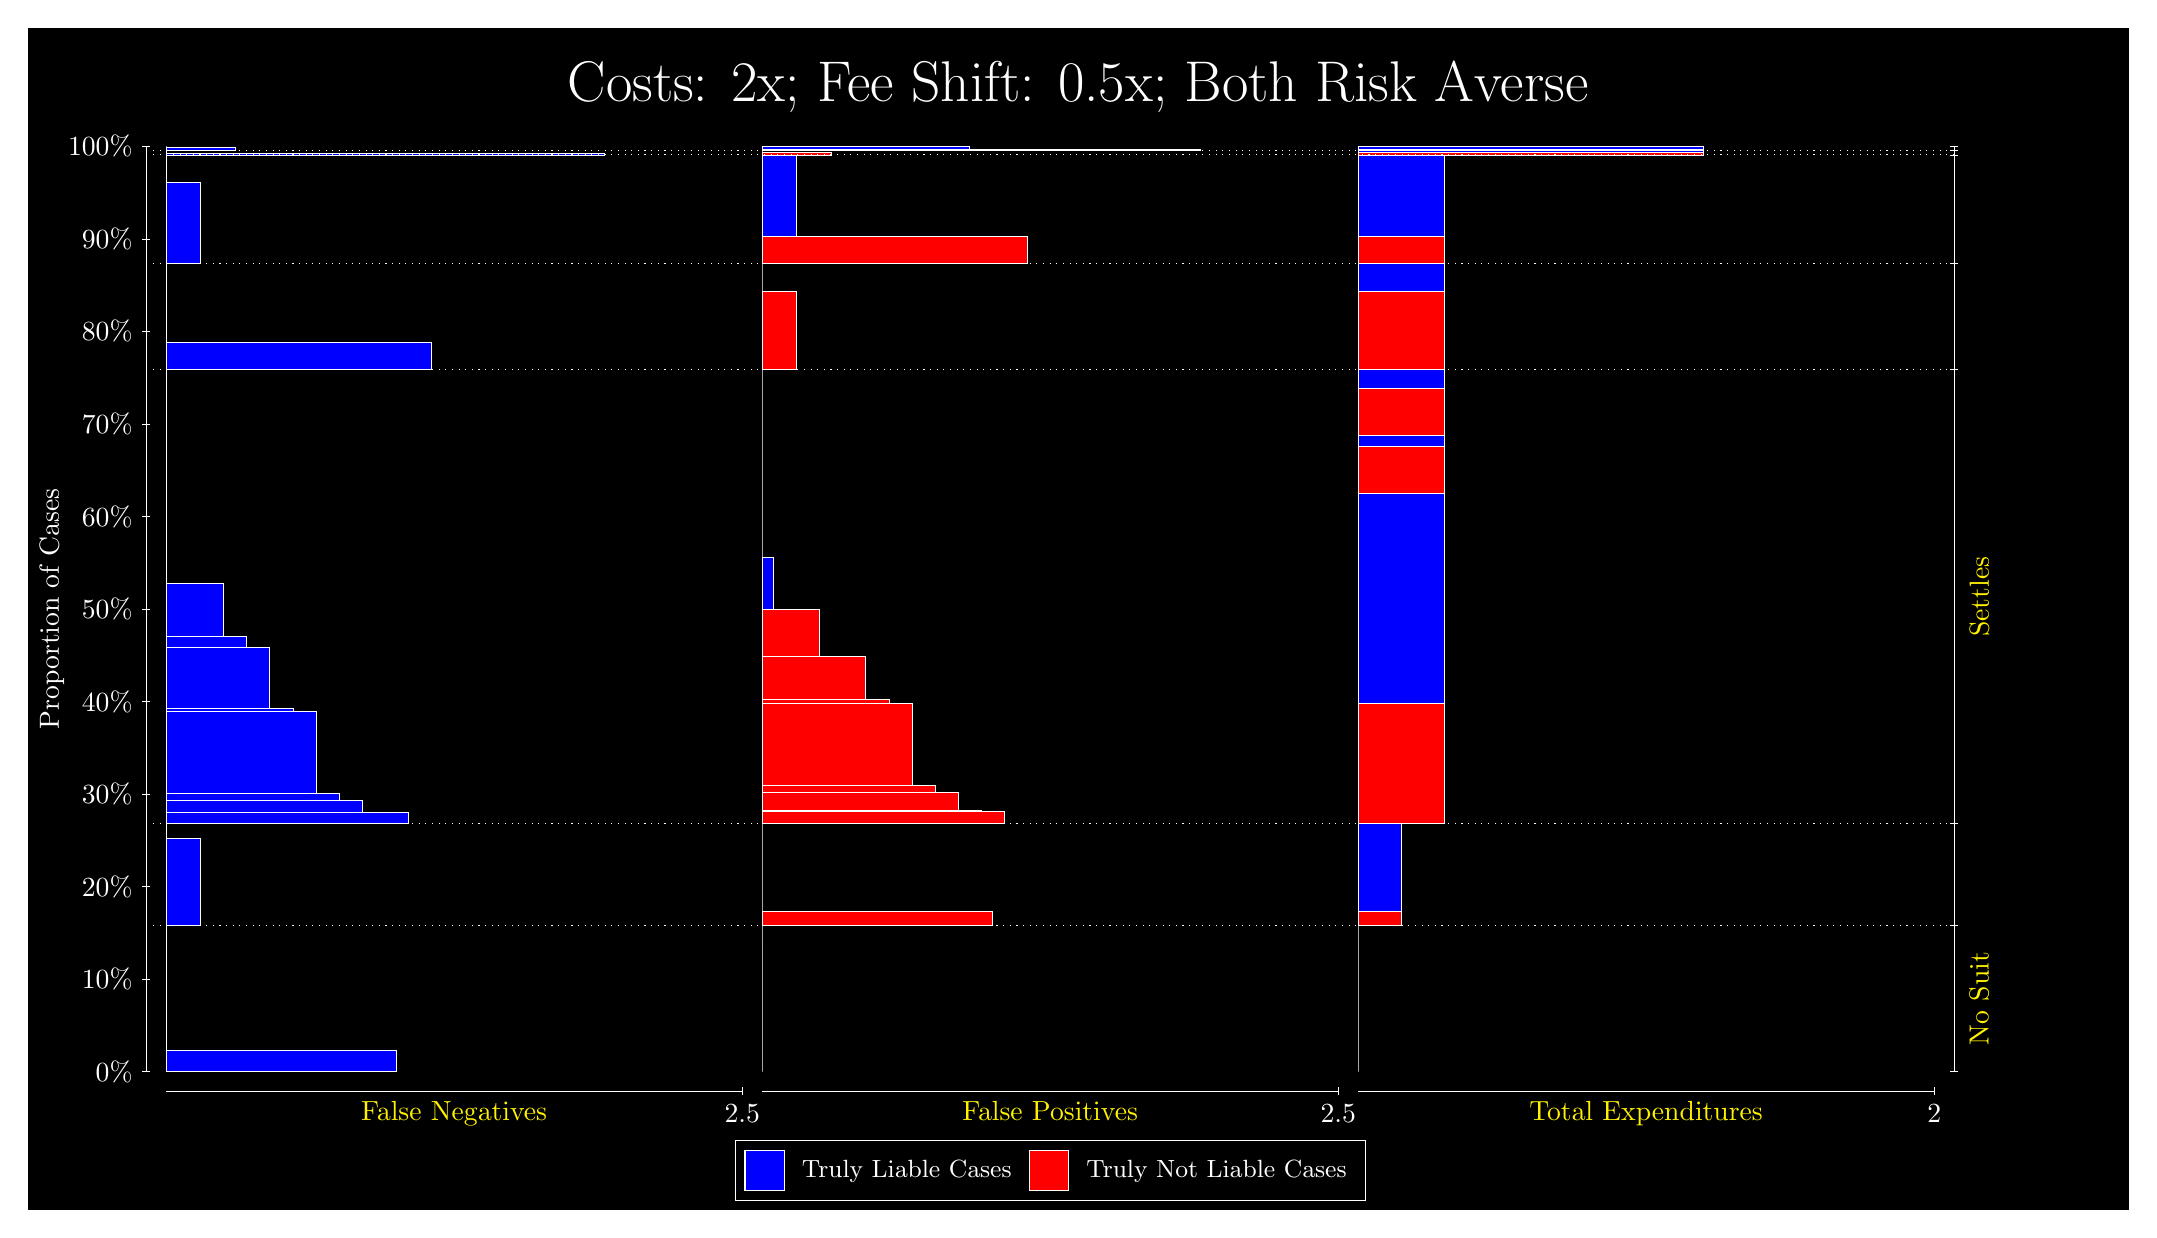
\begin{tikzpicture}
\draw[fill=black] (0,0) rectangle (26.667,15);
\draw[text=white] (0,13.5) rectangle (26.667,15) node[midway] {\huge Costs: 2x; Fee Shift: 0.5x; Both Risk Averse};
\draw[white, very thin] (1.5,1.75) -- (1.5,13.5);
\node[rotate=90, text=white, anchor=center] at (0.3, 7.625) {Proportion of Cases};
\draw[white, very thin] (1.45,1.75) -- (1.55,1.75);
\node[text=white, anchor=east] at (1.45, 1.75) {0\%};
\draw[white, very thin] (1.45,2.925) -- (1.55,2.925);
\node[text=white, anchor=east] at (1.45, 2.925) {10\%};
\draw[white, very thin] (1.45,4.1) -- (1.55,4.1);
\node[text=white, anchor=east] at (1.45, 4.1) {20\%};
\draw[white, very thin] (1.45,5.275) -- (1.55,5.275);
\node[text=white, anchor=east] at (1.45, 5.275) {30\%};
\draw[white, very thin] (1.45,6.45) -- (1.55,6.45);
\node[text=white, anchor=east] at (1.45, 6.45) {40\%};
\draw[white, very thin] (1.45,7.625) -- (1.55,7.625);
\node[text=white, anchor=east] at (1.45, 7.625) {50\%};
\draw[white, very thin] (1.45,8.8) -- (1.55,8.8);
\node[text=white, anchor=east] at (1.45, 8.8) {60\%};
\draw[white, very thin] (1.45,9.975) -- (1.55,9.975);
\node[text=white, anchor=east] at (1.45, 9.975) {70\%};
\draw[white, very thin] (1.45,11.15) -- (1.55,11.15);
\node[text=white, anchor=east] at (1.45, 11.15) {80\%};
\draw[white, very thin] (1.45,12.325) -- (1.55,12.325);
\node[text=white, anchor=east] at (1.45, 12.325) {90\%};
\draw[white, very thin] (1.45,13.5) -- (1.55,13.5);
\node[text=white, anchor=east] at (1.45, 13.5) {100\%};

\draw[white, very thin] (24.457,1.75) -- (24.457,13.5);
\draw[white, very thin] (24.407,1.75) -- (24.507,1.75);
\node[anchor=west] at (24.407, 1.75) {};
\draw[white, very thin] (24.407,3.605) -- (24.507,3.605);
\node[anchor=west] at (24.407, 3.605) {};
\draw[white, very thin] (24.407,4.8984) -- (24.507,4.8984);
\node[anchor=west] at (24.407, 4.8984) {};
\draw[white, very thin] (24.407,10.663) -- (24.507,10.663);
\node[anchor=west] at (24.407, 10.663) {};
\draw[white, very thin] (24.407,12.009) -- (24.507,12.009);
\node[anchor=west] at (24.407, 12.009) {};
\draw[white, very thin] (24.407,13.391) -- (24.507,13.391);
\node[anchor=west] at (24.407, 13.391) {};
\draw[white, very thin] (24.407,13.444) -- (24.507,13.444);
\node[anchor=west] at (24.407, 13.444) {};
\draw[white, very thin] (24.407,13.5) -- (24.507,13.5);
\node[anchor=west] at (24.407, 13.5) {};

\draw[white, very thin, fill=blue] (1.75,1.75) rectangle (4.6775,2.0212);
\draw[white, very thin, fill=red] (1.75,2.0212) rectangle (1.75,3.605);
\draw[white, very thin, fill=blue] (1.75,3.605) rectangle (2.1891,4.7176);
\draw[white, very thin, fill=red] (1.75,4.7176) rectangle (1.75,4.8984);
\draw[white, very thin, fill=blue] (1.75,4.8984) rectangle (4.8239,5.0424);
\draw[white, very thin, fill=blue] (1.75,5.0424) rectangle (4.2384,5.1916);
\draw[white, very thin, fill=blue] (1.75,5.1916) rectangle (3.9457,5.2798);
\draw[white, very thin, fill=blue] (1.75,5.2798) rectangle (3.6529,6.3304);
\draw[white, very thin, fill=blue] (1.75,6.3304) rectangle (3.3602,6.36);
\draw[white, very thin, fill=blue] (1.75,6.36) rectangle (3.0674,7.137);
\draw[white, very thin, fill=blue] (1.75,7.137) rectangle (2.7746,7.2768);
\draw[white, very thin, fill=blue] (1.75,7.2768) rectangle (2.4819,7.9452);
\draw[white, very thin, fill=red] (1.75,7.9452) rectangle (1.75,10.663);
\draw[white, very thin, fill=blue] (1.75,10.663) rectangle (5.1167,11.016);
\draw[white, very thin, fill=red] (1.75,11.016) rectangle (1.75,12.009);
\draw[white, very thin, fill=blue] (1.75,12.009) rectangle (2.1891,13.044);
\draw[white, very thin, fill=red] (1.75,13.044) rectangle (1.75,13.391);
\draw[white, very thin, fill=blue] (1.75,13.391) rectangle (7.3123,13.408);
\draw[white, very thin, fill=red] (1.75,13.408) rectangle (1.75,13.444);
\draw[white, very thin, fill=blue] (1.75,13.444) rectangle (2.6283,13.483);
\draw[white, very thin, fill=red] (1.75,13.483) rectangle (1.75,13.5);
\draw[white, very thin, fill=red] (9.3189,1.75) rectangle (9.3189,3.3338);
\draw[white, very thin, fill=blue] (9.3189,3.3338) rectangle (9.3189,3.605);
\draw[white, very thin, fill=red] (9.3189,3.605) rectangle (12.246,3.7858);
\draw[white, very thin, fill=blue] (9.3189,3.7858) rectangle (9.3189,4.8984);
\draw[white, very thin, fill=red] (9.3189,4.8984) rectangle (12.393,5.0543);
\draw[white, very thin, fill=red] (9.3189,5.0543) rectangle (12.1,5.0734);
\draw[white, very thin, fill=red] (9.3189,5.0734) rectangle (11.807,5.2976);
\draw[white, very thin, fill=red] (9.3189,5.2976) rectangle (11.515,5.3839);
\draw[white, very thin, fill=red] (9.3189,5.3839) rectangle (11.222,6.433);
\draw[white, very thin, fill=red] (9.3189,6.433) rectangle (10.929,6.4721);
\draw[white, very thin, fill=red] (9.3189,6.4721) rectangle (10.636,7.0296);
\draw[white, very thin, fill=red] (9.3189,7.0296) rectangle (10.051,7.6166);
\draw[white, very thin, fill=blue] (9.3189,7.6166) rectangle (9.4652,8.2849);
\draw[white, very thin, fill=blue] (9.3189,8.2849) rectangle (9.3189,10.663);
\draw[white, very thin, fill=red] (9.3189,10.663) rectangle (9.758,11.655);
\draw[white, very thin, fill=blue] (9.3189,11.655) rectangle (9.3189,12.009);
\draw[white, very thin, fill=red] (9.3189,12.009) rectangle (12.686,12.356);
\draw[white, very thin, fill=blue] (9.3189,12.356) rectangle (9.758,13.391);
\draw[white, very thin, fill=red] (9.3189,13.391) rectangle (10.197,13.428);
\draw[white, very thin, fill=blue] (9.3189,13.428) rectangle (9.3189,13.444);
\draw[white, very thin, fill=red] (9.3189,13.444) rectangle (14.881,13.461);
\draw[white, very thin, fill=blue] (9.3189,13.461) rectangle (11.954,13.5);
\draw[white, very thin, fill=red] (16.888,1.75) rectangle (16.888,3.3338);
\draw[white, very thin, fill=blue] (16.888,3.3338) rectangle (16.888,3.605);
\draw[white, very thin, fill=red] (16.888,3.605) rectangle (17.437,3.7858);
\draw[white, very thin, fill=blue] (16.888,3.7858) rectangle (17.437,4.8984);
\draw[white, very thin, fill=red] (16.888,4.8984) rectangle (17.986,6.433);
\draw[white, very thin, fill=blue] (16.888,6.433) rectangle (17.986,9.0983);
\draw[white, very thin, fill=red] (16.888,9.0983) rectangle (17.986,9.6853);
\draw[white, very thin, fill=blue] (16.888,9.6853) rectangle (17.986,9.8294);
\draw[white, very thin, fill=red] (16.888,9.8294) rectangle (17.986,10.426);
\draw[white, very thin, fill=blue] (16.888,10.426) rectangle (17.986,10.663);
\draw[white, very thin, fill=red] (16.888,10.663) rectangle (17.986,11.655);
\draw[white, very thin, fill=blue] (16.888,11.655) rectangle (17.986,12.009);
\draw[white, very thin, fill=red] (16.888,12.009) rectangle (17.986,12.356);
\draw[white, very thin, fill=blue] (16.888,12.356) rectangle (17.986,13.391);
\draw[white, very thin, fill=red] (16.888,13.391) rectangle (21.279,13.428);
\draw[white, very thin, fill=blue] (16.888,13.428) rectangle (21.279,13.444);
\draw[white, very thin, fill=red] (16.888,13.444) rectangle (21.279,13.461);
\draw[white, very thin, fill=blue] (16.888,13.461) rectangle (21.279,13.5);
\draw[white, dotted] (1.5,3.605) -- (24.457,3.605);
\draw[white, dotted] (1.5,4.8984) -- (24.457,4.8984);
\draw[white, dotted] (1.5,10.663) -- (24.457,10.663);
\draw[white, dotted] (1.5,12.009) -- (24.457,12.009);
\draw[white, dotted] (1.5,13.391) -- (24.457,13.391);
\draw[white, dotted] (1.5,13.444) -- (24.457,13.444);
\draw[white, very thin] (1.75,1.5) -- (9.0689,1.5);
\node[text=yellow, anchor=north] at (5.4094, 1.5) {False Negatives};
\draw[white, very thin] (9.0689,1.45) -- (9.0689,1.55);
\node[text=white, anchor=north] at (9.0689, 1.45) {2.5};

\draw[white, very thin] (9.3189,1.5) -- (16.638,1.5);
\node[text=yellow, anchor=north] at (12.978, 1.5) {False Positives};
\draw[white, very thin] (16.638,1.45) -- (16.638,1.55);
\node[text=white, anchor=north] at (16.638, 1.45) {2.5};

\draw[white, very thin] (16.888,1.5) -- (24.207,1.5);
\node[text=yellow, anchor=north] at (20.547, 1.5) {Total Expenditures};
\draw[white, very thin] (24.207,1.45) -- (24.207,1.55);
\node[text=white, anchor=north] at (24.207, 1.45) {2};

\node[text=yellow, centered, rotate=90] at (24.777, 2.6775) {No Suit};

\node[text=yellow, centered, rotate=90] at (24.777, 7.7809) {Settles};





\draw (12.978300999999998,1.5) node[draw=none] (baseCoordinate) {};
\begin{scope}[align=center]
        \matrix[scale=0.5, draw=white, below=0.5cm of baseCoordinate, nodes={draw}, column sep=0.1cm]{
            \node[rectangle, draw, minimum width=0.5cm, minimum height=0.5cm, fill=blue] {}; &
            \node[draw=none, font=\small, text=white] (B) {Truly Liable Cases}; &
            \node[rectangle, draw, minimum width=0.5cm, minimum height=0.5cm, fill=red] {}; &
            \node[draw=none, font=\small, text=white] (B) {Truly Not Liable Cases}; \\
            };
\end{scope}

\end{tikzpicture}
\end{document}